\textit{\textbf{Estimation of Unobservable Geological Characteristics of Horizontal Wells}} --- Not all well-specific information on geological features is available to econometricians. The NDGS geological survey data only include estimates of four different measurements of geological properties at a given location. Because the geospatial data was published to the public in 2008, it is likely that fracking firms, whose objective is to maximize their profits, have already exploited the contents of the maps. As discussed in \cite{Learning-where-to-drill_Agerton_2020}, learning about the spatial distribution of deposits by drilling wells is one of three economic factors that govern firms' where-to-drill decisions. So, it is reasonable to suppose that firms have private information about the Bakken area's spatial distribution of geological characteristics, which is not accessible to researchers. 

The geological characteristics observed only by firms play two different roles in their drilling decisions. First, firms choose whether to drill a location based on its resource quality. Thus, the sample of wells we observe is not random: it has been selected based on unobservable (to us) resource quality. Second, firms' choice of inputs during hydraulic fracturing of each well may be correlated with the unobservable resource quality. For these reasons, accounting for resource quality is critical in modeling firms' decisions and production functions. 

Following \cite{The-Economics-of-Time-Limited-Development-Options_2020_Herrnstadt-Kellogg-and-Lewis}, we employ Robinson's partially linear model to determine the unobservable quality of the horizontal wells completed between 2009 and 2018. We first specify the oil production from a horizontal well as
\begin{equation}
\begin{split}
    \log \left( y_{i} \right) \ 
    & = \ \log \left( \boldsymbol{X}_{i} \right)' \boldsymbol{\beta} \ - \ \lambda \left( longitude_{i}, latitude_{i} \right) \ + \ \epsilon_{i}.
\end{split}
\label{Equation:Production-Function}
\end{equation}
In this specification, $y_{i}$ are horizontal well $i$'s cumulative oil production at its cumulative production month 24.\footnote{That is, unobservable geological features are estimated cross-sectionally in our estimation.} The covariate vector $\boldsymbol{X}_{i}$ for well $i$ includes hydraulic fracturing inputs (i.e., fluid volume, proppant weight, and length of horizontal drilling), cumulative producing days, and observable geological characteristics (i.e., thickness, total organic contents, and thermal maturity). The term $\lambda(longitude_{i}, latitude_{i})$ is a nonparametric function of each well's coordinates and captures well $i$'s unobservable resource quality. Lastly, $\epsilon_{i}$ is a productivity shock not correlated with resource quality. 

To operationalize model (\ref{Equation:Production-Function}), we estimate the following partially linear model:
\begin{equation}
\begin{split}
    \log \left( y_{i} \right) \ - \ \widehat{m}_{y_{i}} \ 
    & = \ \left( \log \left( \boldsymbol{X}_{i} \right) \ - \ \widehat{\boldsymbol{m}}_{\boldsymbol{X}_{i}} \right)' \boldsymbol{\beta} \ + \ \epsilon_{i}.
\end{split}
\label{Equation:Partially-Linear-Model}
\end{equation}
Here, $\widehat{m}_{y_{i}}$ are predictions from a non-parametric regression of $\log \left( y_{i} \right)$ on well $i$'s coordinates $(longitude_{i}, latitude_{i})$. The $\widehat{m}_{y_{i}}$ terms are smoothed means. Differencing these means out serves the same role as the within-transformation in a fixed effects model. In fact, if one used a uniform kernel function, $\widehat{m}_{y_{i}}$, within discrete cells, the estimator would be mathematically identical to fixed effect estimation with spatial fixed effects for each well. Predictions $\widehat{\boldsymbol{m}}_{\boldsymbol{X}_{i}}$ are obtained from different nonparametric regressions whose dependent and independent variables are $\log \left( \boldsymbol{X}_{i} \right)$ and $(longitude_{i}, latitude_{i})$, respectively. The values of primary interest $\widehat{\lambda}_{i}$ (i.e., the unobservable geological quality of horizontal well $i$) are estimated as follows\footnote{For details of Robinson's difference estimator, refer to \textit{9.7.3 Partially Linear Model} in \cite{MicroEconometrics-Methods-and-Applications_Cameron-and-Trivedi_2005}.}:
\begin{equation}
\begin{split}
    \widehat{\lambda}_{i} \
    & = \ \widehat{m}_{y_{i}} \ - \ \widehat{\boldsymbol{m}}_{\boldsymbol{X}_{i}}' \widehat{\boldsymbol{\beta}}
\end{split}
\label{Equation:Estimates}
\end{equation}
\afterpage{
    \begin{figure}[t!]
        \centering
        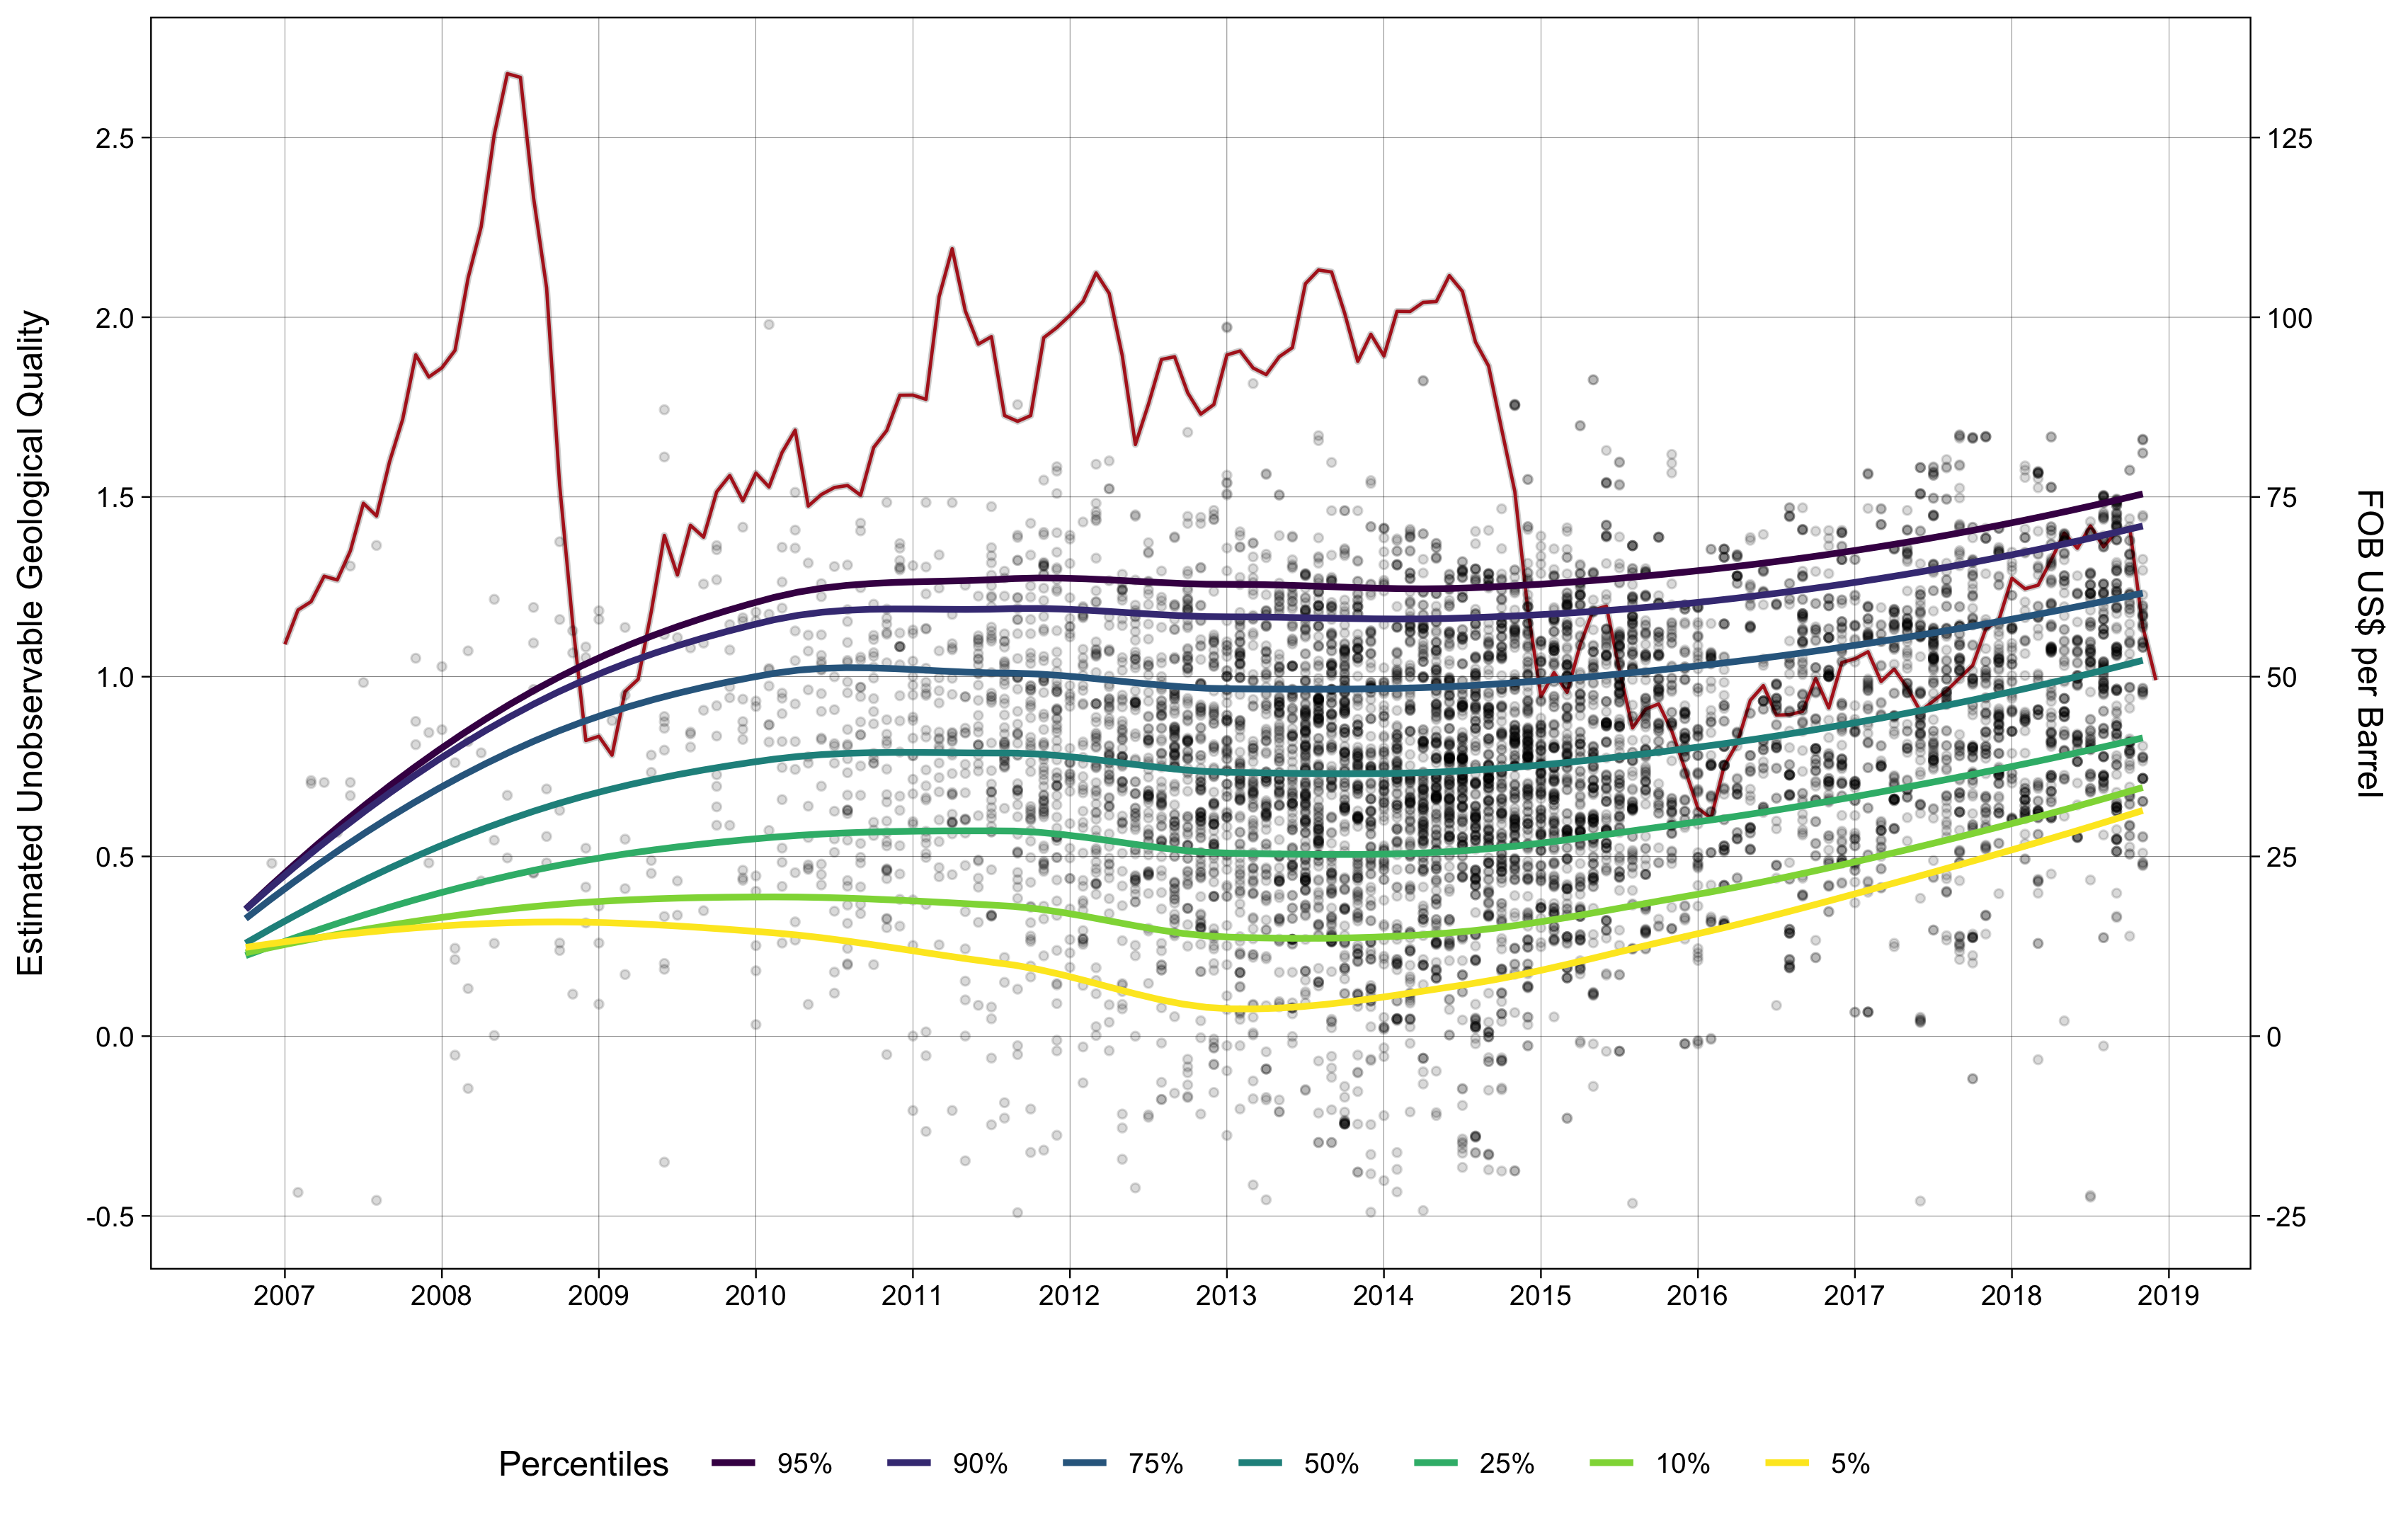
\includegraphics[scale = 0.13]{04_Chapter-3/00A_Figures/Figure_Cross-Sectional-Approach_Estimates-from-Robinson-Estimator_Time-Trend-of-Unobservable-Geological-Quality.png}
        \caption{Simultaneous Drilling of Horizontal Wells with Heterogeneous Geological Quality}
        \caption*{
            {\small
            \textit{Note}: 
            This figure indicates the estimated geological feature for each horizontal well, depicted as a dot. Those dots definitely suggest the simultaneous drilling of horizontal wells with heterogeneous geological quality. In the figure, percentiles of the estimates, with the 95\% confidence interval of each, are also presented. The solid red line is the time series of the monthly per-barrel spot prices for West Texas Intermediate at Cushing, Oklahoma. Oil prices plunged significantly between 2014 and 2015 and rose gradually. The percentile lines skewed upward, especially lower ones, as of the second half of 2014.  
        }}
        \label{Figure:Simultaneous-Drilling-of-Horizontal-Wells-with-Heterogeneous-Geological-Quality}
    \end{figure}
}
In our analysis, we define low- and high-quality locations by dividing our sample of well sites into those with $\widehat{m}_{y_{i}}$ below and above the median. Even though $\widehat{m}_{y_{i}}$ is estimated from only higher-quality locations with observed drilling, and therefore biased upward, the ordinal ranking of well sites should be affected less. Figure \ref{Figure:Spatial-Distribution-of-the-Estimated-Geological-Characteristic-by-Year} shows the spatial distribution of the estimated quality.
